\documentclass[conference]{IEEEtran}
\usepackage[english]{babel}
\usepackage{graphicx}
\usepackage{amsmath,amssymb}
\usepackage{algorithm,algpseudocode}
\usepackage{booktabs}
\usepackage{cite}
\usepackage{hyperref}
\usepackage{xcolor}

\hypersetup{colorlinks=true,linkcolor=blue,citecolor=blue,urlcolor=blue}

\begin{document}

\title{Shanghai Metro Line Planning:\\
Reproduction and Line-Pool Selection}

\author{
\IEEEauthorblockN{Yuzhou Lu, Zaizhou Yang, Jingrong Guan}
\IEEEauthorblockA{ShanghaiTech University\\
CS240 -- Algorithm Design and Analysis\\
\{luyzh, yangzzh2025, guanjr2022\}@shanghaitech.edu.cn}
}

\maketitle

\begin{abstract}
This paper studies urban rail line planning through both algorithm
reproduction and a compact line-selection framework of our own. We first
reproduce two representative TNDP methods: the greedy extension and
insertion heuristics of Laporte et al.\ (2005) for single-alignment trip
coverage maximization, and the GIS-integrated genetic algorithm of Ahmed
et al.\ (2020) for simultaneous multi-line station and alignment
optimization. We then propose Candidate Line-Pool Selection (CLPS), which
reduces computation by generating plausible lines in advance and selecting
from this finite pool using Greedy-OD, Greedy-BCR, GA-pool, and ILP
selectors. All methods are evaluated on a 54-station Shanghai candidate
graph derived from OpenStreetMap data. The reproduction results confirm
the polynomial runtime scaling predicted by complexity analysis and show
that simultaneous multi-line optimization outperforms individual line
optimization by 18\%. CLPS-Greedy-OD reaches 51.9\% OD coverage in only
0.01 s, demonstrating the value of reducing route design to line-pool
selection. The best OD coverage overall is achieved by Laporte H2-C
(56.8\%), while multi-line methods provide better transfer structure and
operational flexibility.
\end{abstract}

\begin{IEEEkeywords}
transit network design, line-pool selection, greedy heuristics, genetic algorithm, OD demand capture, Shanghai metro
\end{IEEEkeywords}

%--------------------------------------------------------------------------
\section{Introduction}
%--------------------------------------------------------------------------

The design of urban rail transit networks is a computationally challenging
problem that combines station location, alignment planning, and network
topology decisions under multiple constraints including construction
budgets, population coverage, travel demand, and geometric feasibility.
Formally known as the Transit Network Design Problem (TNDP), it is NP-hard
in the general case, motivating the development of practical heuristics.

This paper has two goals. The first is reproduction: we implement two
influential algorithms from the TNDP literature that represent
complementary approaches to the problem. Laporte et al.\ (2005) formulate
the single-alignment problem as maximizing origin-destination (OD) trip
coverage under a length budget, and propose simple greedy heuristics that
run in polynomial time. Ahmed et al.\ (2020) extend the scope to multi-line
networks by integrating GIS-based feasibility screening with a genetic
algorithm (GA) that simultaneously optimizes station locations and line
alignments.

The second goal is our own reduced-search planning framework. Directly
searching over all ordered station sequences and multi-line combinations is
expensive even for a moderate 54-station candidate set. We therefore build
Candidate Line-Pool Selection (CLPS): a two-stage framework that first
generates plausible lines on a corridor graph and then selects a small
network from this pool. All methods are tested on a realistic dataset
derived from OpenStreetMap (OSM) for central Shanghai.

We contribute: (1) a faithful implementation of the Laporte 2005 greedy
extension and insertion heuristics with incremental effectiveness
computation; (2) an adapted implementation of the Ahmed 2020 GA with
hub-based terminal selection and geometric quality constraints; (3) a CLPS
framework with Greedy-OD, Greedy-BCR, GA-pool, and ILP selectors; and (4) a
unified comparison of reproduction methods and CLPS methods on coverage,
runtime, transfer, detour, and passenger-flow metrics.

%--------------------------------------------------------------------------
\section{Related Work}
%--------------------------------------------------------------------------

\subsection{Overview of TNDP Methods}

The Transit Network Design Problem (TNDP) has been studied since the 1970s
\cite{vuchic1968}, with four main objective classes: (1) maximizing coverage,
(2) minimizing travel time, (3) minimizing cost, and (4) multi-objective
combinations. Early work by Dufourd et al.\ (1996) and Bruno et al.\
(2002) applied Tabu search to single-line population coverage. Laporte et
al.\ (2005) shifted to OD trip coverage with polynomial greedy
heuristics---our first reproduction target. On the multi-line front, Chai
et al.\ (2019) used simulated annealing, while Ahmed et al.\ (2020)
combined GIS feasibility screening with a GA for simultaneous multi-line
optimization---our second target. The line-pool approach of Sch\"{o}bel and
Scholl (2005) motivates our CLPS framework: instead of searching directly
over all possible station sequences, we generate a manageable pool of
plausible candidate lines and solve a smaller line-selection problem.

\subsection{Laporte et al.\ (2005): Single Alignment Maximization}

Given candidate stations $S$ with trip coverage values $f_{ij}$ and a
logit mode-choice function $g_{ij}(E)$, the MTCP seeks an ordered subset
$E \subseteq S$ maximizing ridership subject to length budget $L_{\max}$:
\begin{equation}
\begin{aligned}
\max_{E \subseteq S} \quad & \sum_{i,j \in E} n_{ij}(E) \\
\text{s.t.} \quad
& n_{ij}(E) = f_{ij} \cdot g_{ij}(E), \\
& \text{Length}[\text{Align}(E)] \leq L_{\max}.
\end{aligned}
\label{eq:mtcp}
\end{equation}
This generalizes the bounded-length Hamiltonian path problem (NP-hard).

The paper proposes two constructive heuristics: \textbf{H1 (Greedy
Extension)} starts from the best station pair and repeatedly extends at
either endpoint; \textbf{H2 (Greedy Insertion)} inserts the best
unselected station at its optimal position, with variants A/B/C differing
in selection criterion (max ridership, min length, max ratio). A
\textbf{post-optimization} step reinserts each station at its best
position until convergence.

With incremental effectiveness computation, H1 runs in $O(n^3)$ and H2 in
$O(n^4)$, where $n = |S|$. Post-optimization costs $O(k^3)$ per pass.

\subsection{Ahmed et al.\ (2020): Integrated Multi-Line Optimization}

Ahmed et al.\ minimize total system cost:
\begin{equation}
\min \; T_c = \phi_p P_c + \phi_o O_c + \phi_c C_c
\label{eq:ahmed_obj}
\end{equation}
where $P_c$, $O_c$, $C_c$ are passenger, operator, and community costs.
Stage~1 uses GIS to screen feasible station cells; Stage~2 applies a GA
with tournament selection, uniform crossover, and station-level mutation.
Chromosomes encode entire solutions (lines as genes, stations as bits);
terminals are pre-specified. Constraints include 4--7 stations per line,
800--1500 m spacing, and $\leq$30\% line overlap. Total complexity is
$O(N_{\text{cells}} K + G \cdot P \cdot L \cdot N_s^2 \log N_s)$.

%--------------------------------------------------------------------------
\section{Data, Reproduction, and CLPS Implementation}
%--------------------------------------------------------------------------

\subsection{Data Pipeline}

Following the project proposal, we separate spatial data preparation from
the route-optimization stage. The optimization algorithms do not operate
directly on raw GIS layers. Instead, their common input is a prepared
candidate-station set
$V=\{1,\ldots,n\}$, where each station $i$ has a coordinate
$p_i=(\lambda_i,\phi_i)$ and a nonnegative value $v_i$. Candidate edges are
then assigned geographic construction lengths $\ell_{ij}$, and the
optimization stage searches for ordered station sequences or multi-line
subgraphs over this reduced spatial graph.

We instantiate this proposal pipeline using public OpenStreetMap (OSM) data
for central Shanghai (121.40--121.56$^\circ$E, 31.14--31.26$^\circ$N).
First, we extract building footprints and functional OSM features such as
commercial, office, retail, university, hospital, transport, and amenity
points. Residential population is estimated from building footprint area
under a fixed study-area total of 300k residents, while job and activity
weights are assigned from the functional features. Second, we form candidate
urban centers by running weighted $k$-means on population, job, and
commercial/activity weights, and add three fixed high-importance hubs to
ensure that major urban anchors are retained. Nearby centers within
1,000 m are merged, producing a final 54-station candidate set with station
values ranging from 30k to 635k.

Third, we convert the station set into a feasible planning graph. Rather
than using the complete graph for every algorithm, we build an
MST-plus-short-edges corridor graph: the minimum spanning tree preserves
global connectivity, while additional short station pairs provide local
alignment alternatives. This graph supplies edge lengths, shortest-path
distances, and geometric constraints for the CLPS and GA methods.
Finally, because real census OD data are unavailable, we generate a
gravity-model demand proxy
$\text{OD}_{ij} \propto \text{pop}_i^{1.5} \cdot \text{jobs}_j / d_{ij}^\gamma$.
Thus the final prepared dataset consists of station coordinates, station
values, corridor edges, edge lengths, and an OD matrix shared by all
reproduced algorithms and CLPS methods.

\begin{figure}[!t]
\centering
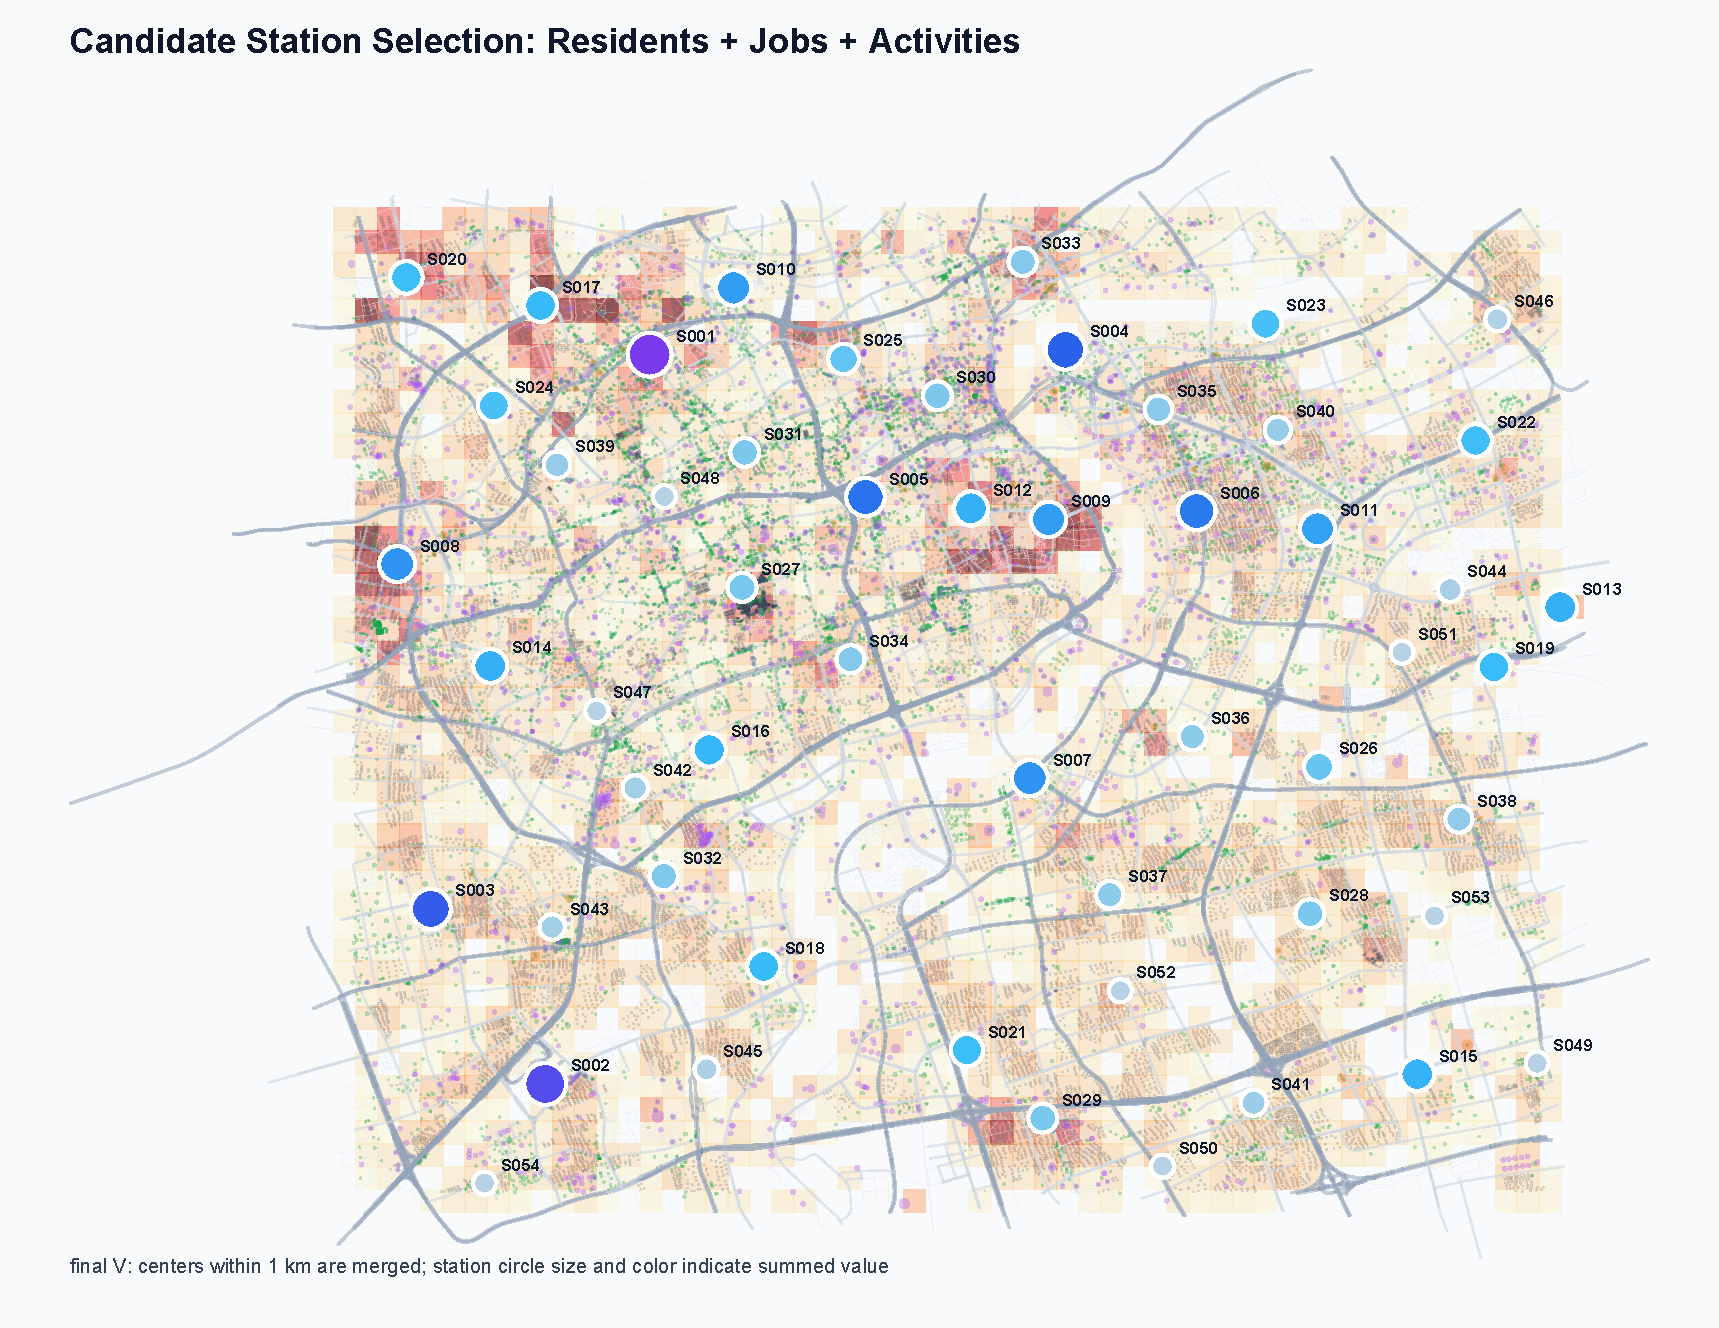
\includegraphics[width=\columnwidth]{figures/station_selection.pdf}
\caption{Final 54 candidate stations generated from the Shanghai OSM
preprocessing pipeline. Marker size reflects the station value used by the
optimization algorithms.}
\label{fig:station_selection}
\end{figure}

\subsection{Laporte 2005 Implementation}

We implement H1, H2-A/B/C, and post-optimization in 334 lines of Python,
using incremental effectiveness computation ($O(|P|)$ gain per station
addition). Three simplifications from the original: (1) gravity-model OD
replaces census-tract trip coverage (justified by the paper's statement
that heuristics are model-independent); (2) $g_{ij}(E)=1$ (no logit mode
choice); (3) linear distance-decay $E(P)=\sum_{i<j} v_i v_j
\max(0,1-D^P_{ij}/C)$ to make path ordering meaningful.

\subsection{Ahmed 2020 Implementation}

We implement the Stage~2 GA in 829 lines of Python with these adaptations:
(1) our station pipeline replaces GIS grid screening (54 vs.\ 4,774
candidates); (2) data-driven hub-based terminal selection (first line uses
highest-OD pair, subsequent lines share a terminal) replaces planner-specified
terminals; (3) shortest-path initialization on the corridor graph replaces
random sequences; (4) three mutation operators (swap, insert, remove) with
feasibility checks; (5) value-connection fitness replaces the paper's
life-cycle cost model; (6) spacing constraints relaxed for our sparse layout.

\subsection{Candidate Line-Pool Selection}

In addition to the two reproduced algorithms, we implement a third family
of methods called \textbf{Candidate Line-Pool Selection (CLPS)}. Its purpose
is to reduce computation. Directly optimizing metro lines over 54 stations
requires searching over a very large space of ordered station sequences and
multi-line combinations. CLPS decomposes this into two smaller stages:
first generate a finite pool of plausible lines, then select a subset of
lines under optional line-count and budget constraints.

The line pool is generated on the MST-plus-short-edges corridor graph. We
combine three sources of candidate sequences: (1) shortest paths between
the top 120 OD-demand station pairs; (2) shortest paths between pairs among
the top 20 high-value terminal candidates; and (3) 200 biased random walks
that start from value-weighted stations and prefer short corridor edges.
All sequences are filtered to 4--18 stations (random-walk lines use at most
12 stations), reversed duplicates are removed, and each remaining line is
annotated with length, construction cost, covered population, and direct OD
coverage.

\begin{figure}[t]
\centering
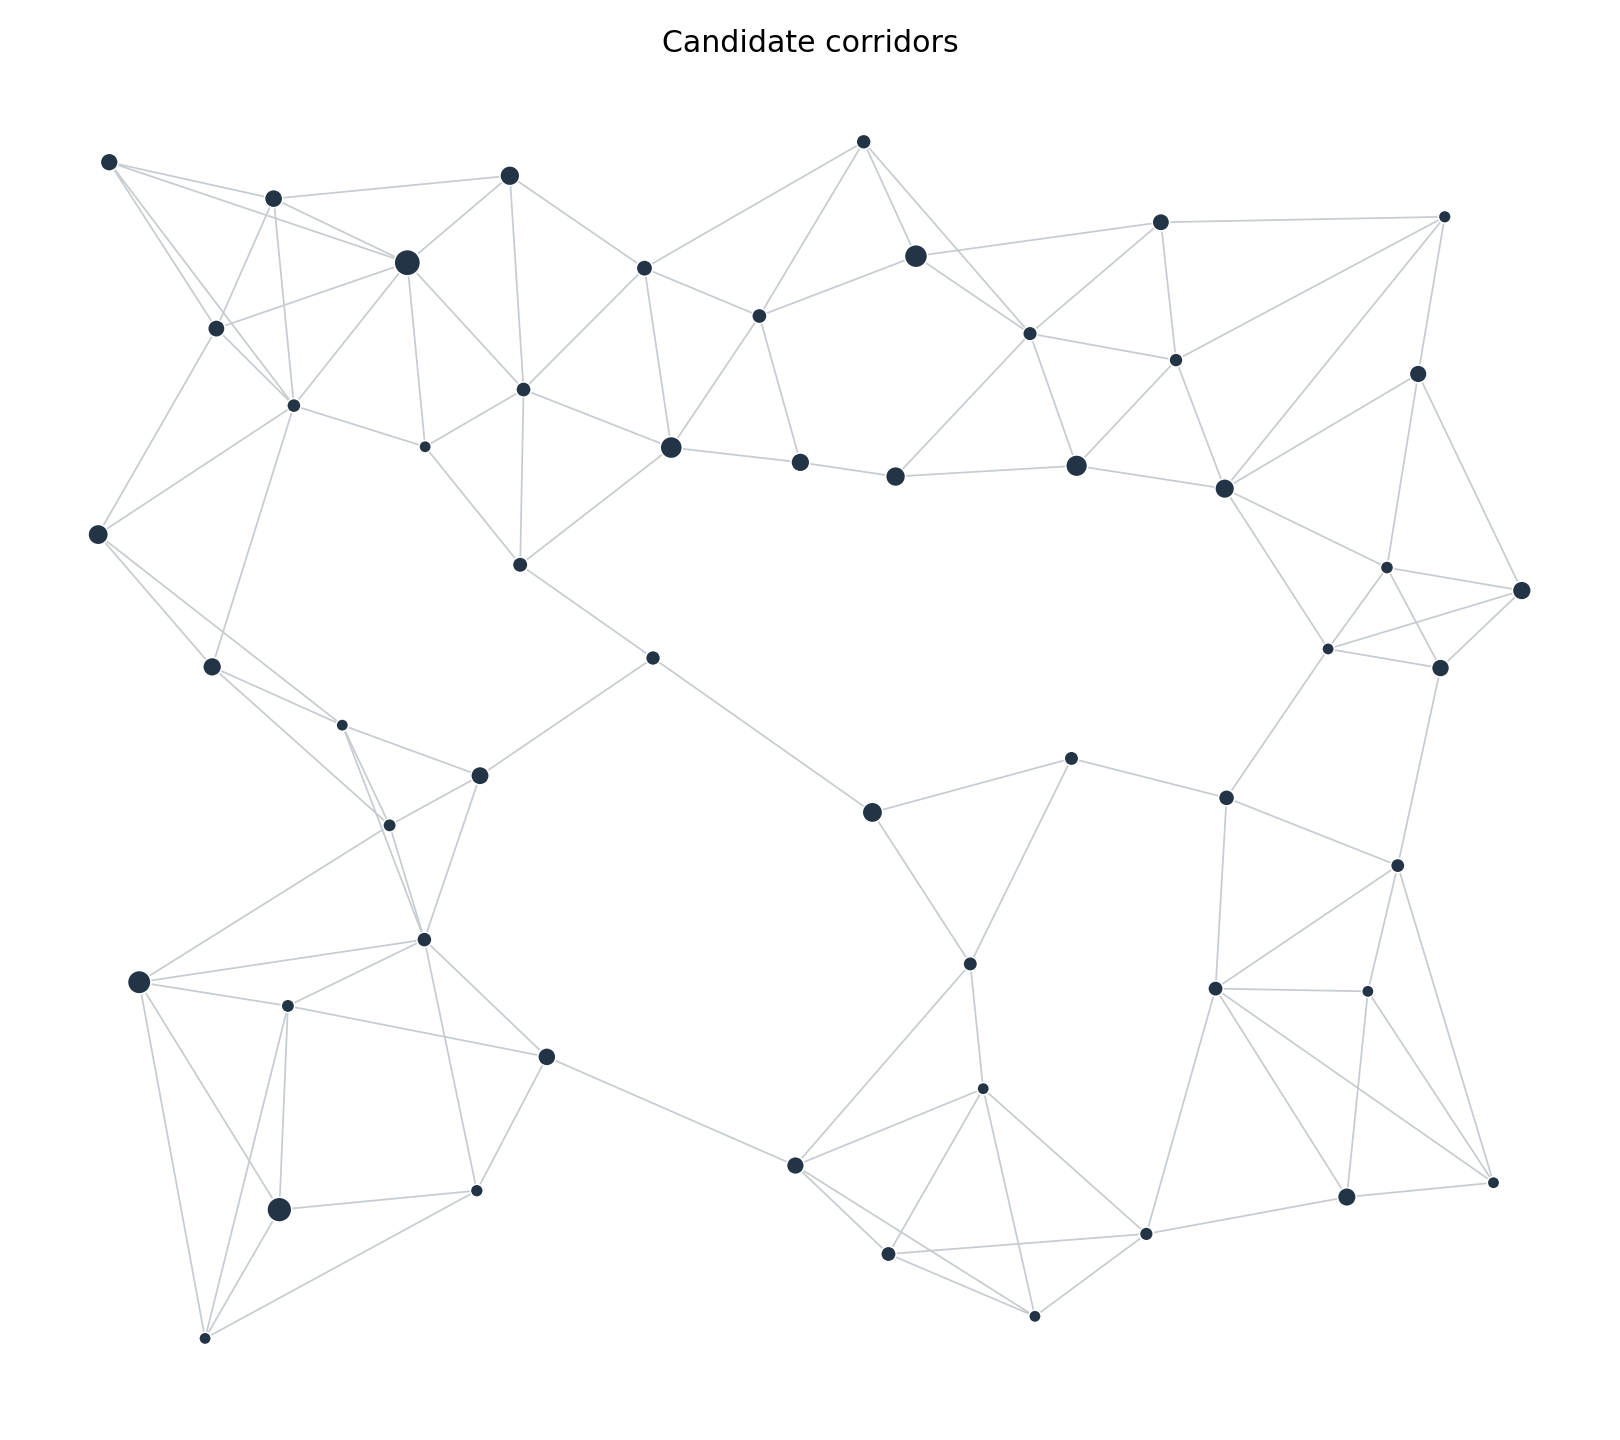
\includegraphics[width=\columnwidth]{figures/clps_candidate_corridors.png}
\caption{Intermediate CLPS corridor graph used for candidate line-pool
generation. Gray edges show the MST-plus-short-edges planning graph from
which shortest-path and random-walk candidate lines are sampled.}
\label{fig:clps_corridors}
\end{figure}

We then solve the reduced line-selection problem with four selectors:
\textbf{Greedy-OD} repeatedly chooses the line with the largest marginal
new direct OD coverage; \textbf{Greedy-BCR} chooses the largest marginal
coverage per construction cost; \textbf{GA-pool} uses a binary chromosome
over candidate lines with crossover, mutation, and a fitness combining OD
coverage, population, station coverage, connectivity, and cost; and
\textbf{ILP} uses binary line variables to maximize direct OD coverage with
optional maximum-line and budget constraints via CBC. CLPS is used only as
our own reduced-search planning framework; the Laporte and Ahmed
reproductions do not depend on the line pool.

\begin{figure}[!t]
\centering
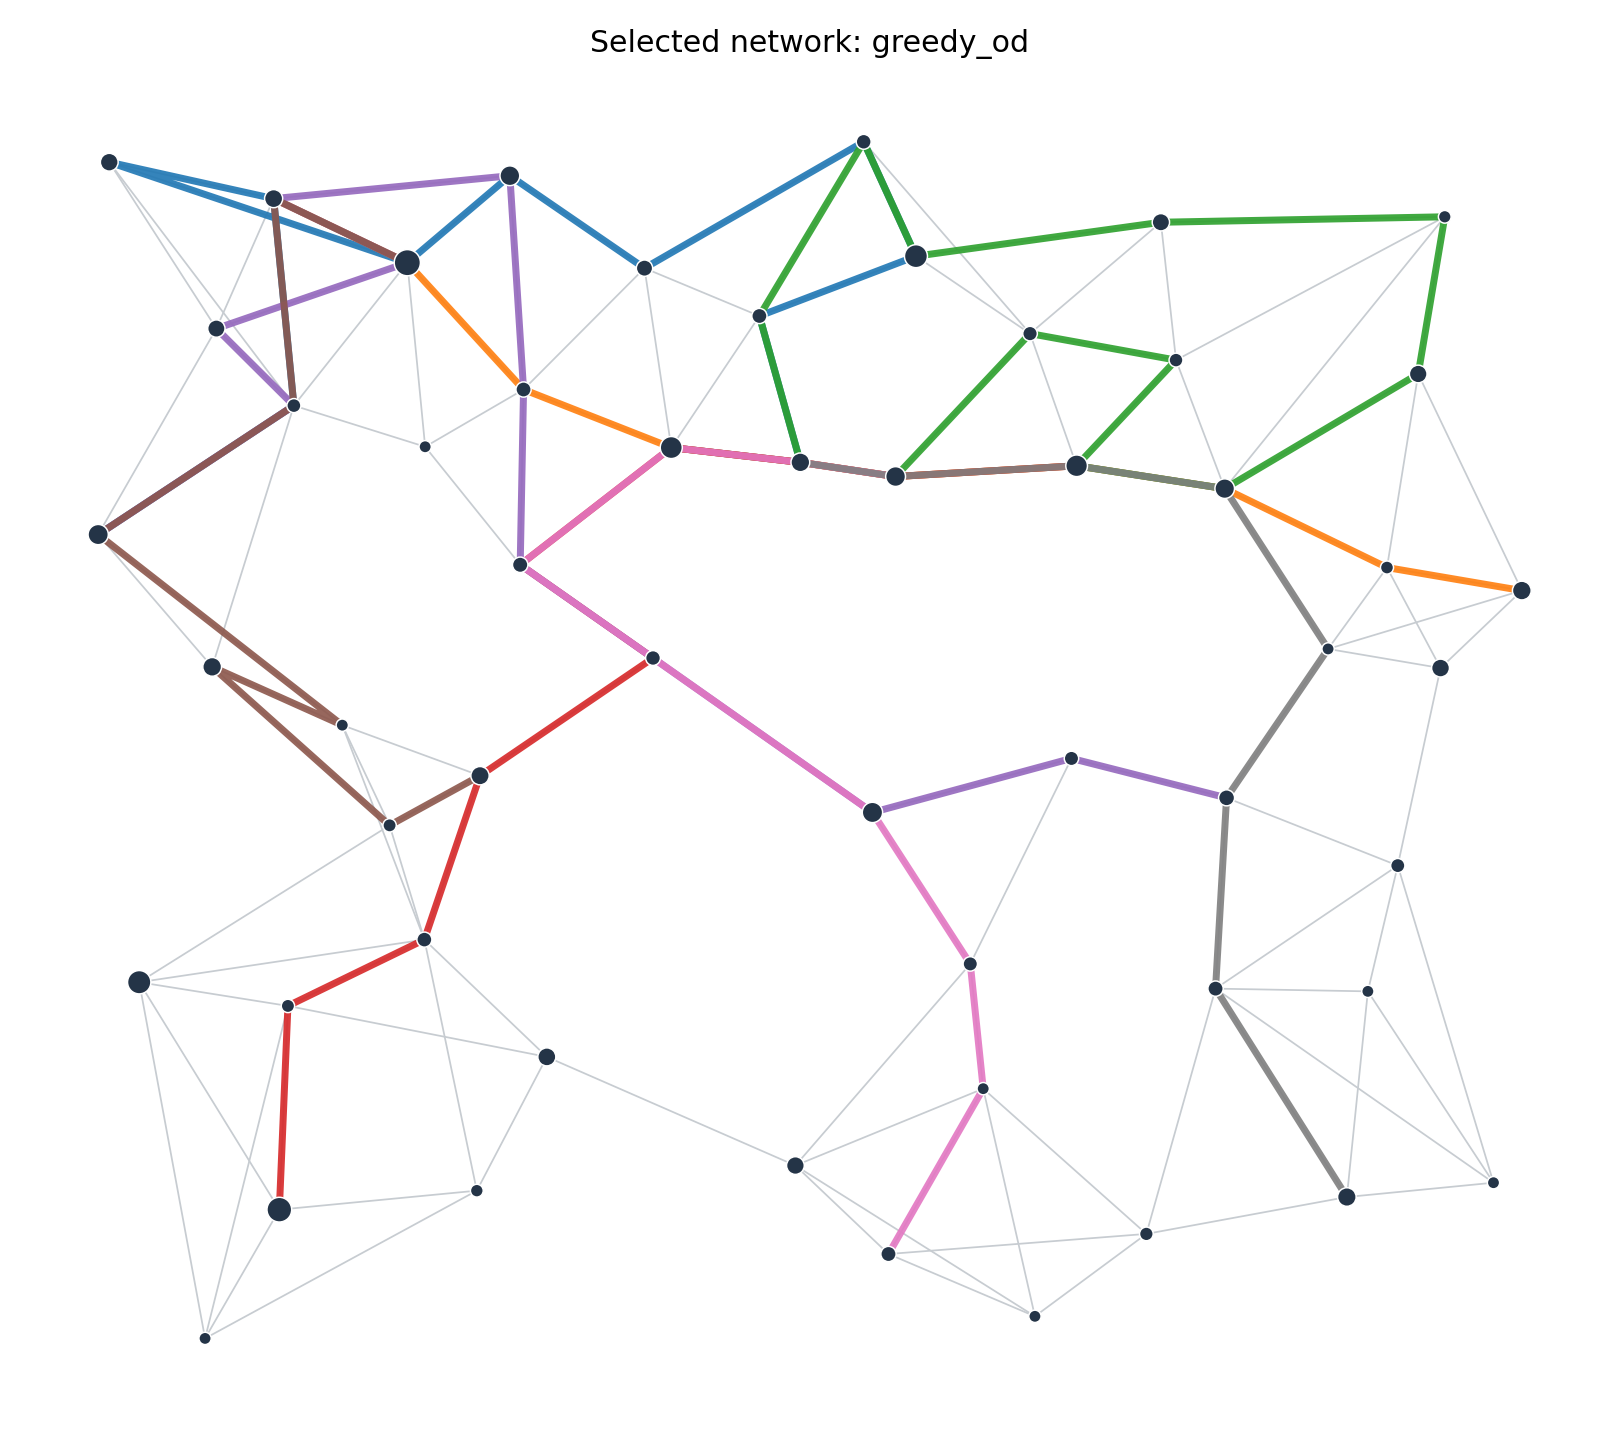
\includegraphics[width=0.98\columnwidth]{figures/clps_network_greedy_od.png}\\[-2pt]
\small (a) CLPS-Greedy-OD

\vspace{3pt}
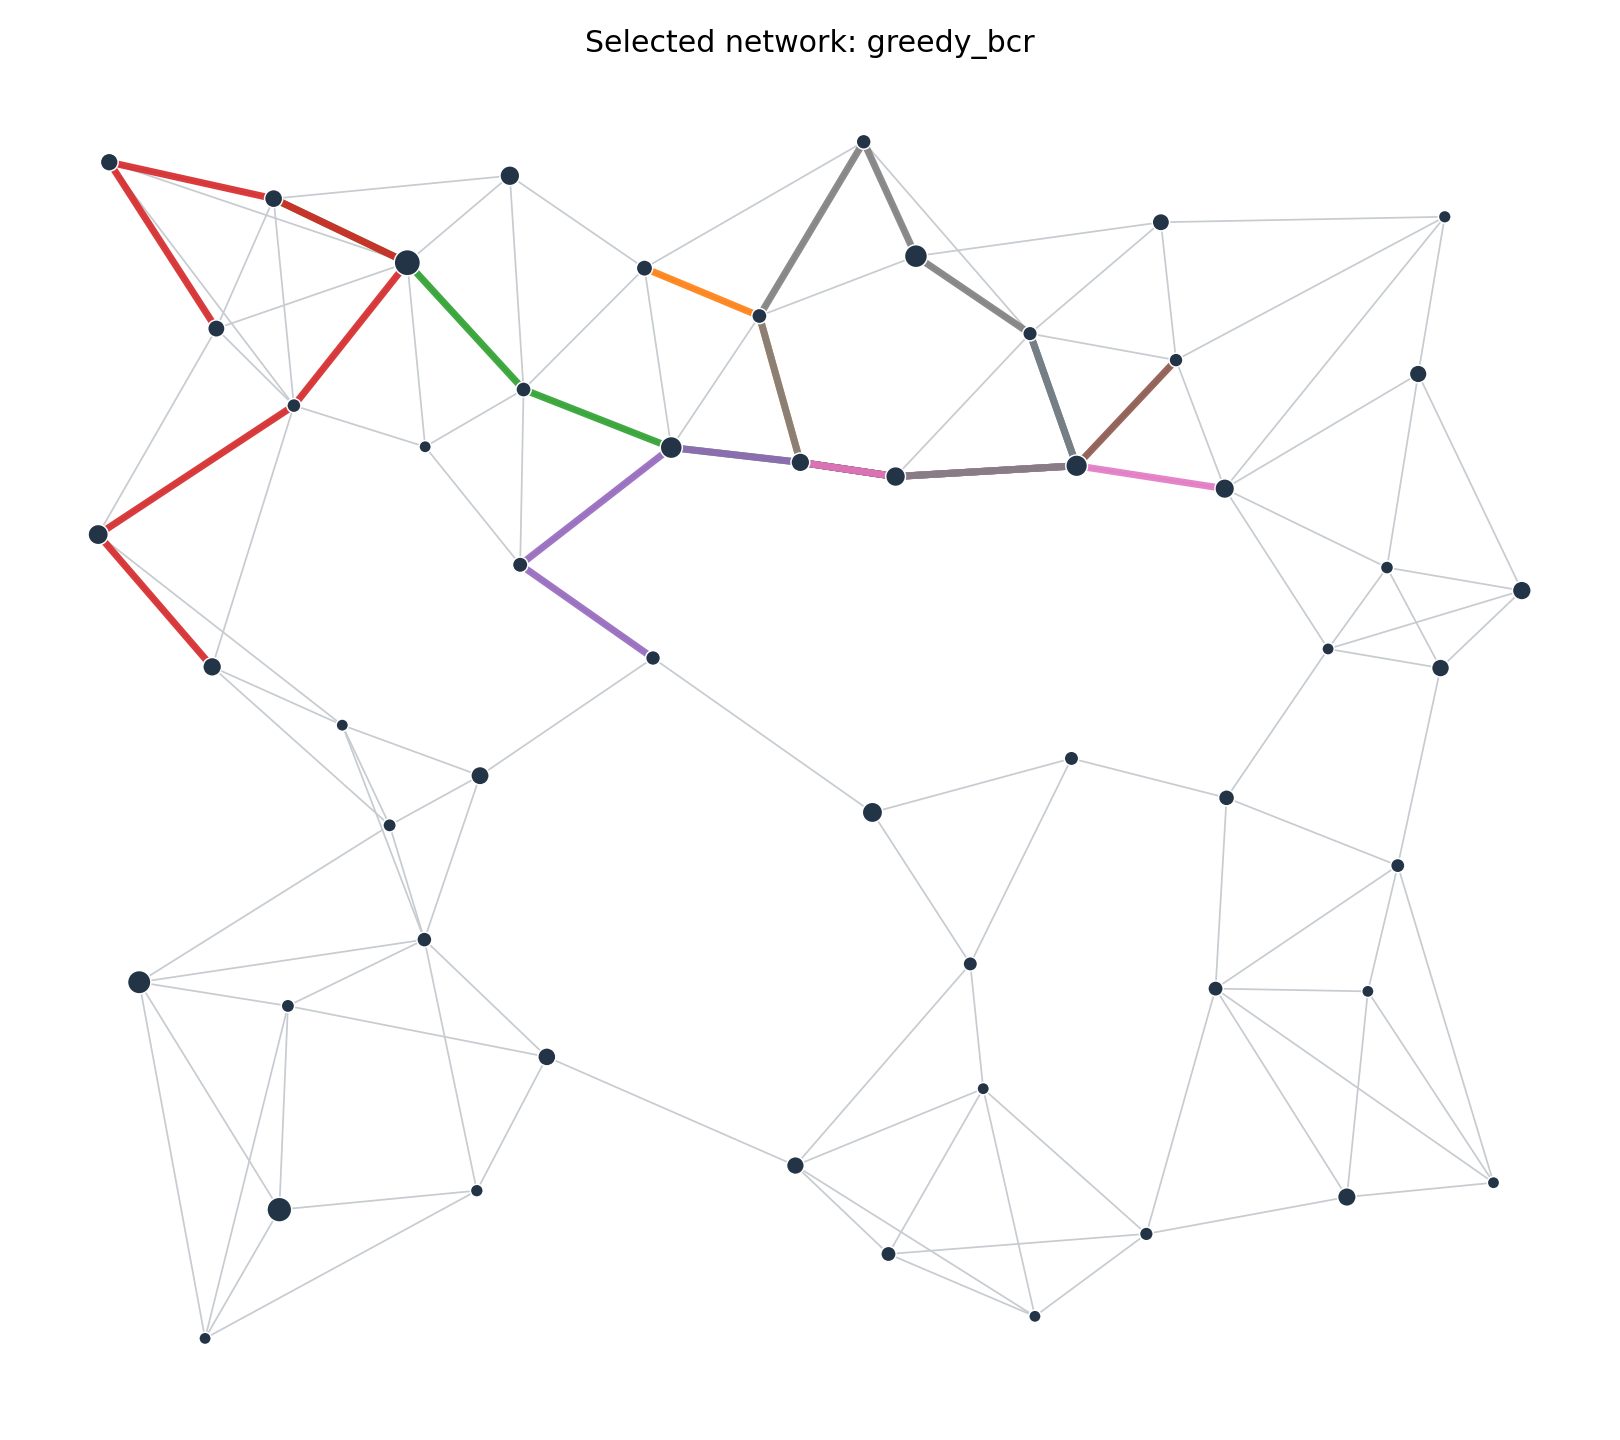
\includegraphics[width=0.98\columnwidth]{figures/clps_network_greedy_bcr.png}\\[-2pt]
\small (b) CLPS-Greedy-BCR
\caption{Greedy CLPS selected networks from the same candidate line pool.
Greedy-OD maximizes marginal direct OD coverage, while Greedy-BCR favors
shorter high-benefit-per-cost lines.}
\label{fig:clps_greedy_networks}
\end{figure}

\begin{figure}[!t]
\centering
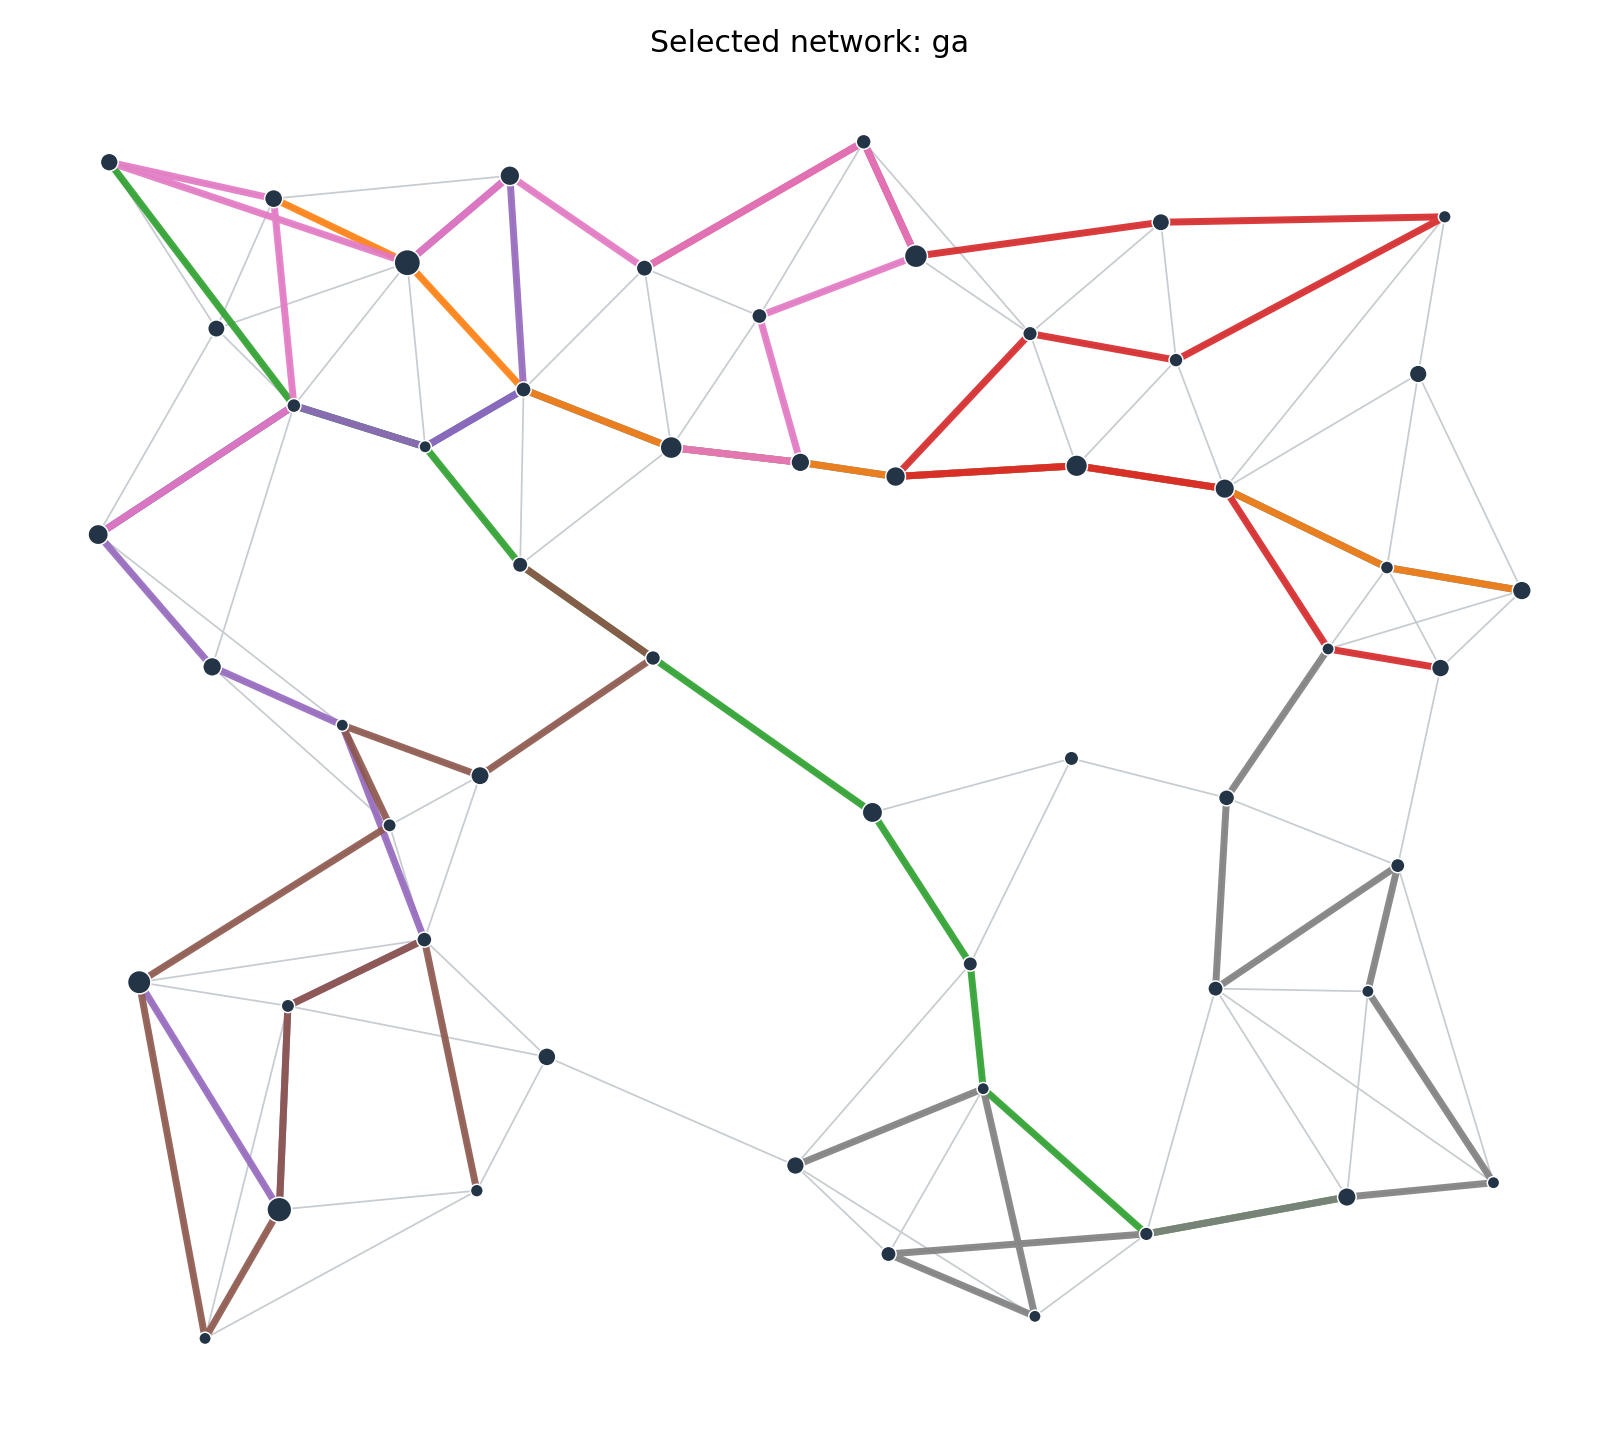
\includegraphics[width=0.98\columnwidth]{figures/clps_network_ga.png}\\[-2pt]
\small (a) CLPS-GA-pool

\vspace{3pt}
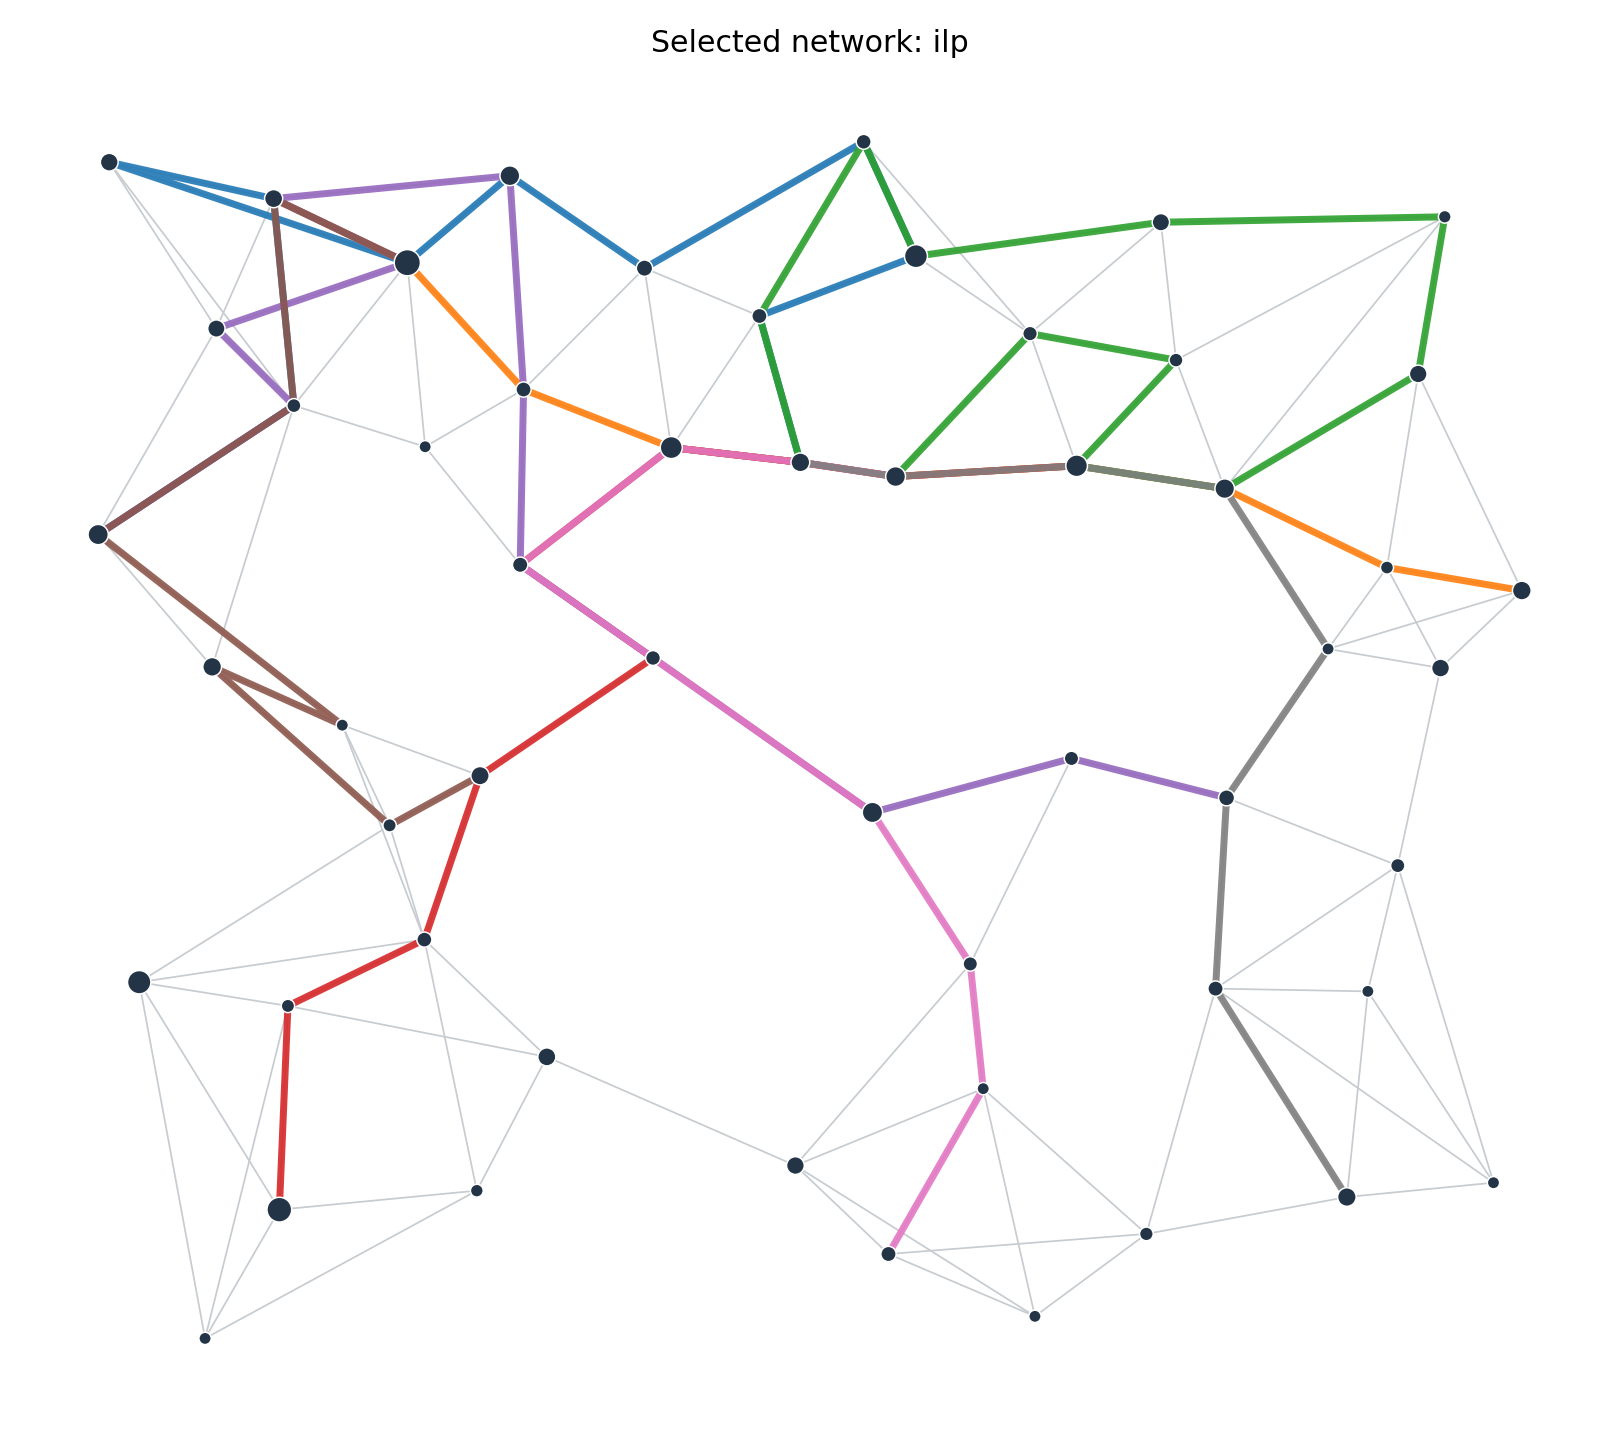
\includegraphics[width=0.98\columnwidth]{figures/clps_network_ilp.png}\\[-2pt]
\small (b) CLPS-ILP
\caption{Optimization-based CLPS selected networks. GA-pool explores broader
population and connectivity trade-offs, while ILP selects the same line set
as Greedy-OD in this run.}
\label{fig:clps_selected_networks}
\end{figure}

%--------------------------------------------------------------------------
\section{Evaluation and Cross-Method Comparison}
%--------------------------------------------------------------------------

\subsection{Laporte 2005 Reproduction}

Table~\ref{tab:laporte_table1} reproduces the paper's Table~1 structure on
our Shanghai dataset with three length budgets.

\begin{table}[t]
\centering
\caption{Laporte 2005 Table~1 reproduction on Shanghai data.}
\label{tab:laporte_table1}
\scriptsize
\setlength{\tabcolsep}{3pt}
\begin{tabular}{lrrrrr}
\toprule
$L_{\max}$ & Method & Len.\ (km) & Ridership & Ratio & T (s) \\
\midrule
40 & H1       & 39.9 & $4.10\!\times\!10^{12}$ & $1.03\!\times\!10^{8}$ & 0.03 \\
40 & H2-A     & 39.6 & $1.04\!\times\!10^{13}$ & $2.61\!\times\!10^{8}$ & 0.31 \\
40 & H2-C     & 39.2 & $1.08\!\times\!10^{13}$ & $2.75\!\times\!10^{8}$ & 0.38 \\
60 & H1       & 59.8 & $6.22\!\times\!10^{12}$ & $1.04\!\times\!10^{8}$ & 0.05 \\
60 & H2-A     & 59.9 & $1.37\!\times\!10^{13}$ & $2.29\!\times\!10^{8}$ & 0.79 \\
60 & H2-C     & 59.6 & $1.36\!\times\!10^{13}$ & $2.28\!\times\!10^{8}$ & 0.93 \\
80 & H1       & 79.3 & $7.60\!\times\!10^{12}$ & $9.59\!\times\!10^{7}$ & 0.08 \\
80 & H2-A     & 80.0 & $1.52\!\times\!10^{13}$ & $1.90\!\times\!10^{8}$ & 1.45 \\
80 & H2-C     & 79.0 & $1.47\!\times\!10^{13}$ & $1.86\!\times\!10^{8}$ & 1.56 \\
\bottomrule
\end{tabular}
\end{table}

\textbf{Deviation from the paper:} The original paper reports H1 dominates
H2 on simulated data. Our results show the opposite: H2-A outperforms H1
by 2--2.5$\times$. This is because without logit mode choice, OD capture
depends on the \emph{set} of stations rather than \emph{ordering}; H2
packs more stations (31 vs.\ 18 at $L_{\max}\!=\!60$ km) by inserting
anywhere in the alignment. Post-optimization yields negligible improvement,
consistent with the paper.

\subsection{Runtime Scalability}

\begin{figure}[t]
\centering
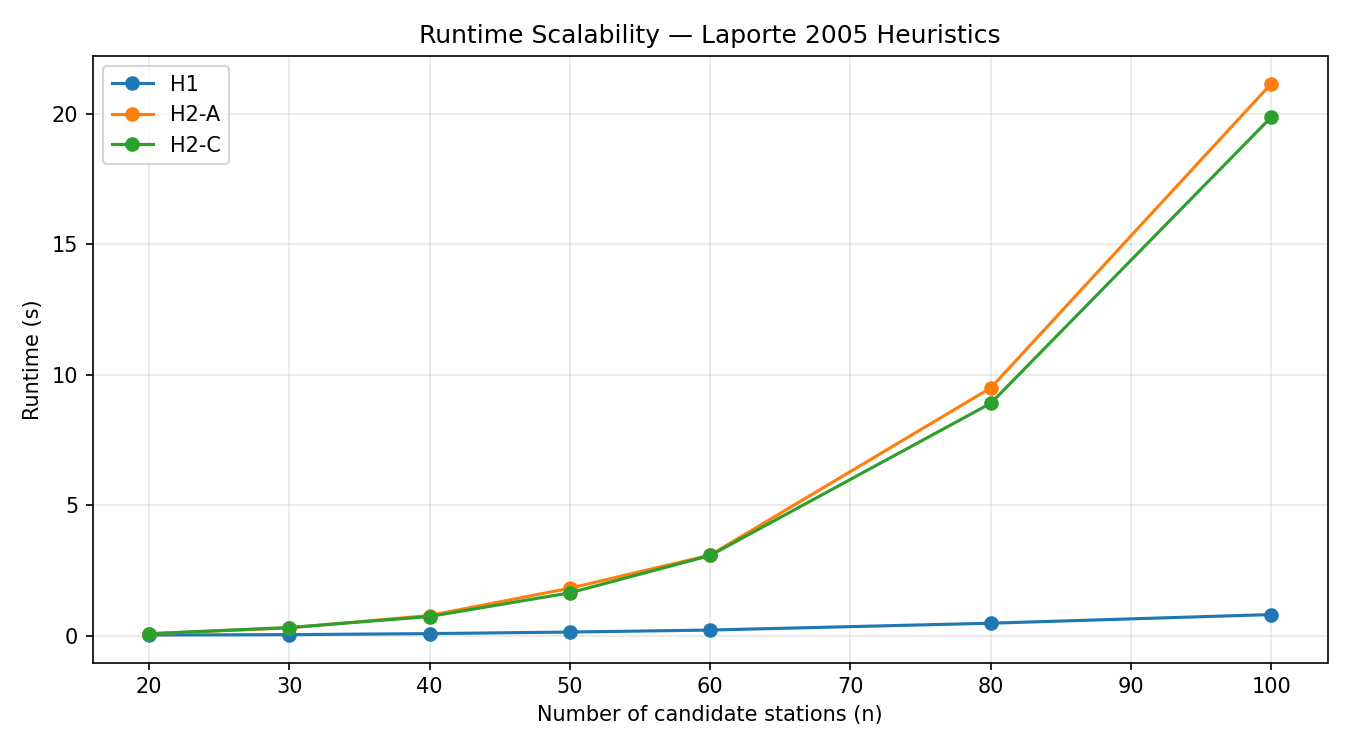
\includegraphics[width=\columnwidth]{figures/runtime_scalability.png}
\caption{Runtime scaling: H1 as $O(n^3)$, H2 as $O(n^4)$, matching
complexity analysis.}
\label{fig:scalability}
\end{figure}

Figure~\ref{fig:scalability} confirms the predicted scaling: H1 runs in
0.02 s at $n\!=\!20$ and 0.81 s at $n\!=\!100$; H2-A in 0.07 s and 21.2 s
respectively. All runtimes are consistent with the paper's conclusion that
``computational times are always insignificant.''

\subsection{Ahmed 2020: Multi-Line Results}

\begin{figure}[t]
\centering
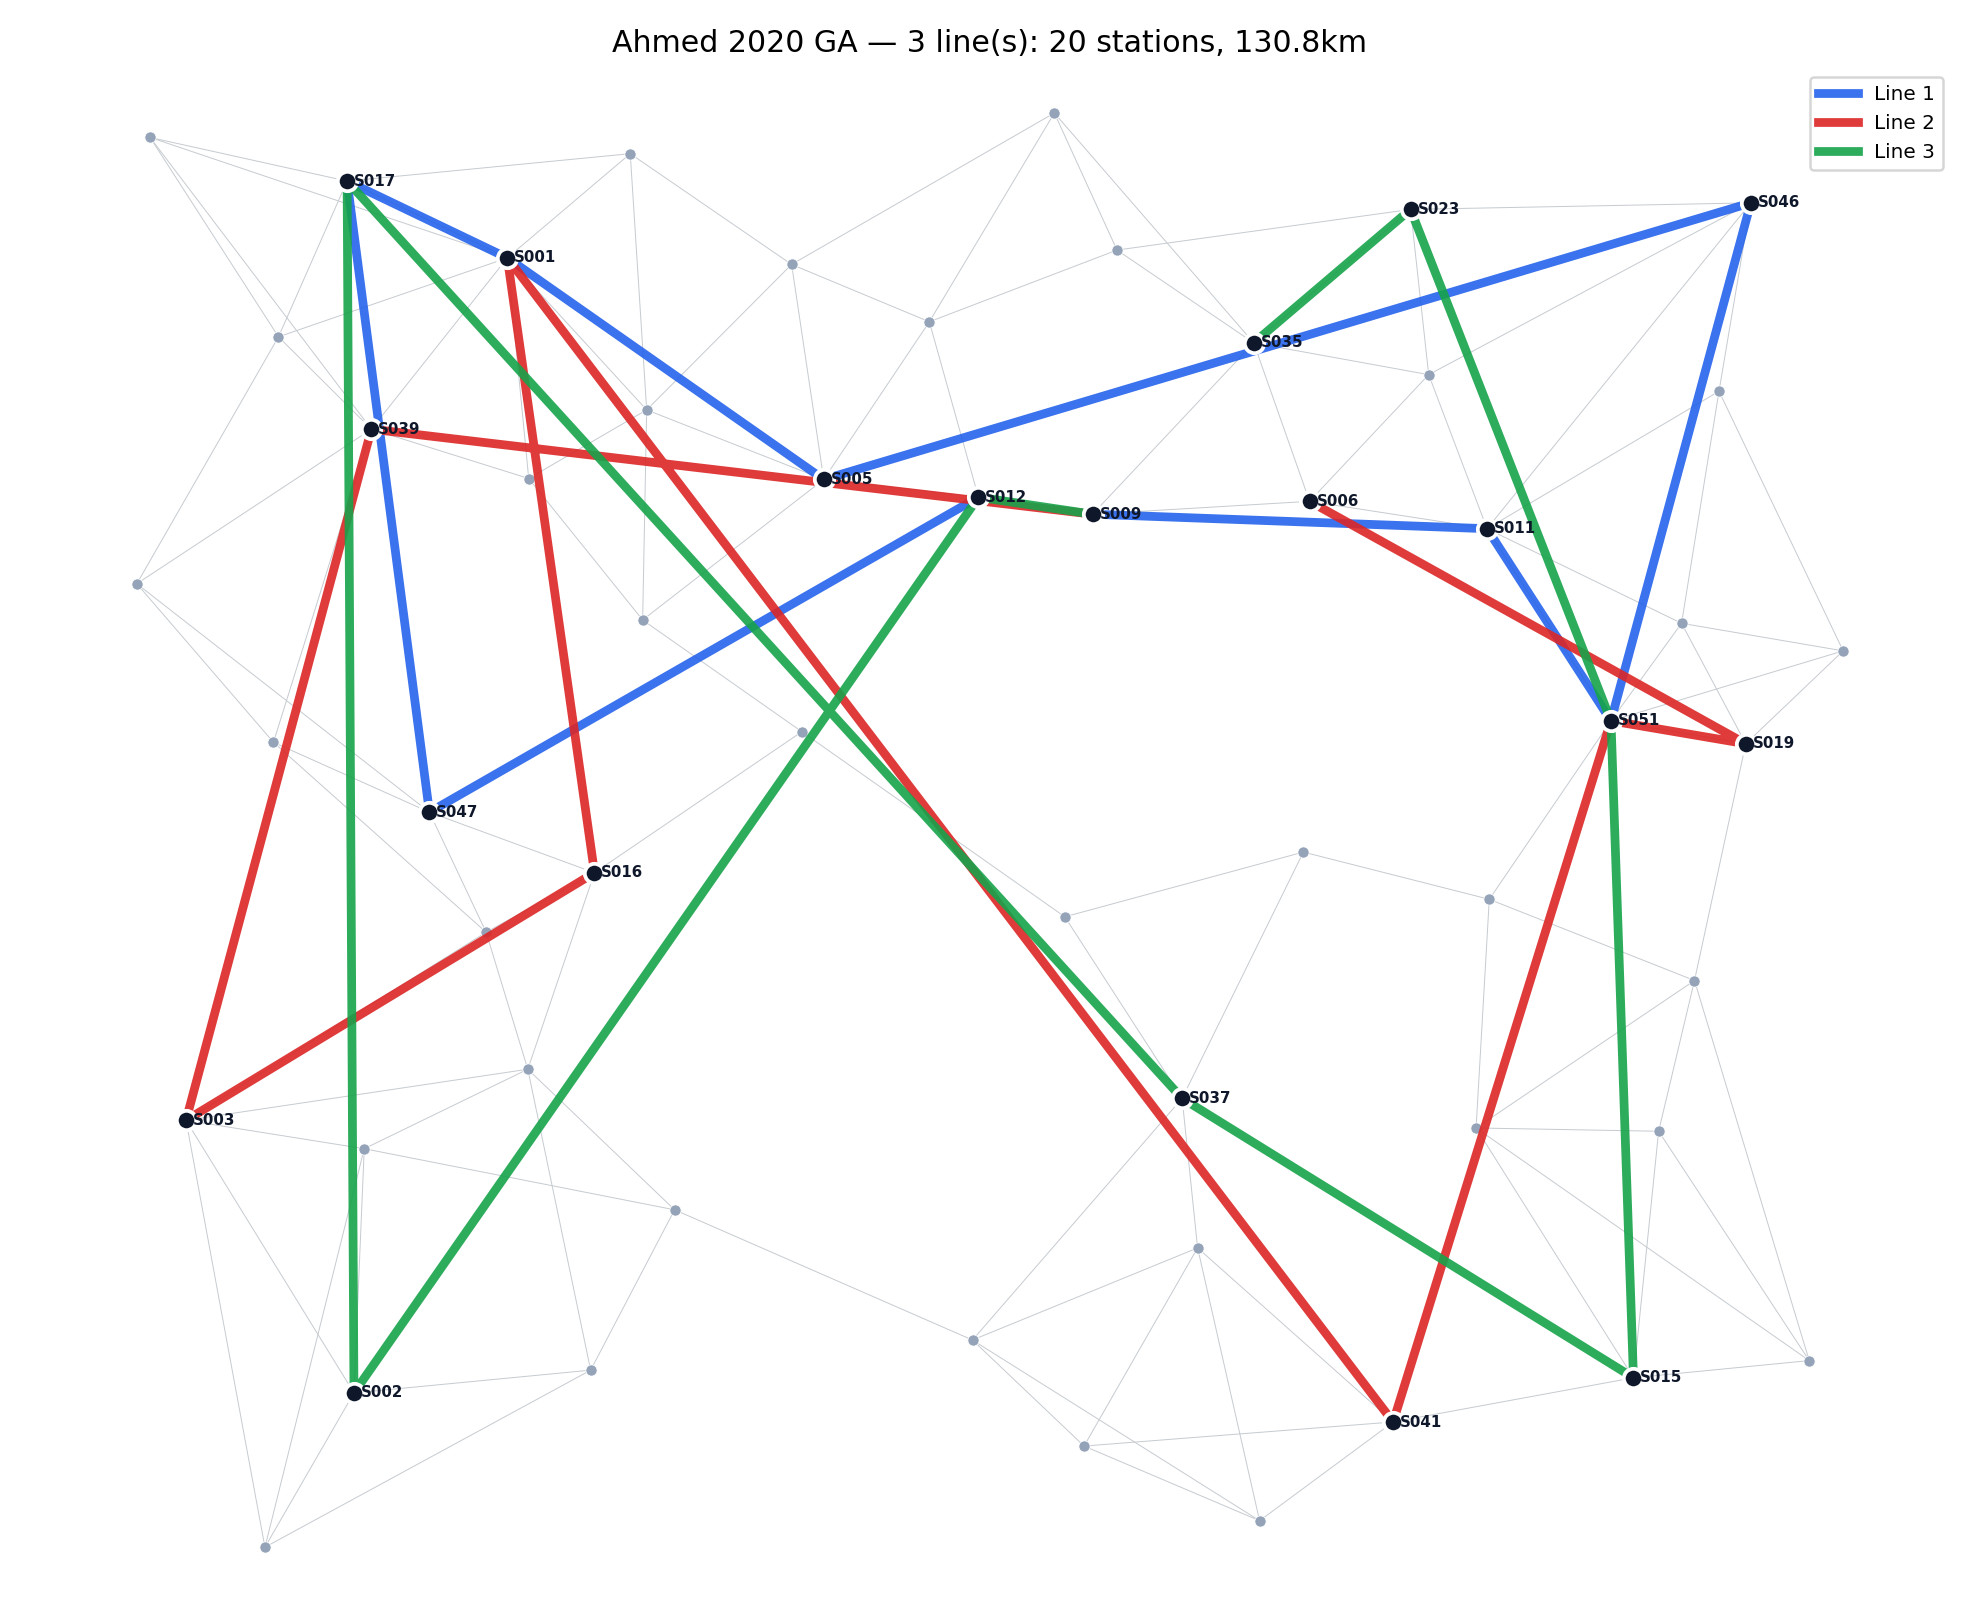
\includegraphics[width=\columnwidth]{figures/ahmed_3line.png}
\caption{3-line GA result: hub-based radial topology centered on S009.}
\label{fig:ahmed_3line}
\end{figure}

Figure~\ref{fig:ahmed_3line} shows the optimized 3-line network with
hub-based radial topology. Table~\ref{tab:ahmed_results} summarizes GA
results. Simultaneous optimization achieves 18\% better cost than
individual optimization (Table~\ref{tab:sim_vs_ind}), consistent with the
paper's qualitative finding, though smaller than its 70\% margin due to
our smaller candidate set (54 vs.\ 4,774).

\begin{table}[t]
\centering
\caption{Ahmed 2020 GA results.}
\label{tab:ahmed_results}
\small
\begin{tabular}{lrrrr}
\toprule
Lines & Stations & Length (km) & Cost & Time (s) \\
\midrule
1 & 14 & 37.0 & $-5.63\!\times\!10^{12}$ & 33.9 \\
2 & 23 & 85.7 & $-1.33\!\times\!10^{13}$ & 57.1 \\
3 & 20 & 130.8 & $-5.81\!\times\!10^{12}$ & 59.6 \\
\bottomrule
\end{tabular}
\end{table}

\begin{table}[t]
\centering
\caption{Simultaneous vs.\ individual optimization (2 lines).}
\label{tab:sim_vs_ind}
\small
\begin{tabular}{lrrrr}
\toprule
Method & Cost & Stations & Len.\ (km) & T (s) \\
\midrule
Simultaneous & $-1.33\!\times\!10^{13}$ & 23 & 85.7 & 58.3 \\
Individual   & $-1.13\!\times\!10^{13}$ & 28 & 80.1 & 68.9 \\
\bottomrule
\end{tabular}
\end{table}

\subsection{CLPS Line-Pool Evaluation}

We separately evaluate CLPS on the generated candidate line pool. After
deduplication and length filtering, the pool contains 400 candidate lines.
Their lengths range from 3.9 km to 26.3 km, with an average of 10.8 km;
each line contains 4--12 stations, averaging 6.7 stations. This confirms
the intended reduction: instead of searching over all possible station
sequences, the selectors operate on a compact but diverse set of plausible
lines.

\begin{table}[t]
\centering
\caption{CLPS selector results on the 400-line candidate pool
($K_{\max}=8$).}
\label{tab:clps_results}
\scriptsize
\setlength{\tabcolsep}{2.5pt}
\begin{tabular}{lrrrrrr}
\toprule
Selector & Lines & Sta. & Len. & Pop. & OD & Net. \\
 & & & (km) & Cov. & Cov. & Cov. \\
\midrule
Greedy-OD  & 8 & 42 & 101.2 & 90.0\% & \textbf{68.5\%} & 87.9\% \\
Greedy-BCR & 8 & 21 & 35.4  & 67.9\% & 52.1\% & 69.0\% \\
GA-pool    & 8 & 50 & 120.6 & \textbf{97.9\%} & 67.7\% & \textbf{96.3\%} \\
ILP        & 8 & 42 & 101.2 & 90.0\% & \textbf{68.5\%} & 87.9\% \\
\bottomrule
\end{tabular}
\end{table}

Table~\ref{tab:clps_results} shows three clear behaviors. Greedy-OD and
ILP select the same line set in this run, indicating that the greedy
marginal OD rule reaches the direct-OD optimum for this pool and constraint
setting. Greedy-BCR produces the most compact network, using only 35.4 km
of unique track, but sacrifices coverage. GA-pool selects a broader network
that covers 50 stations and achieves the highest network OD coverage
(96.3\%), at the cost of longer track length and slightly larger weighted
detour. These results support the motivation for CLPS: once the route
space is reduced to a candidate line pool, different selectors can explore
coverage-cost trade-offs at very low computational cost.

\subsection{Cross-Method Comparison}

\begin{table}[!t]
\centering
\caption{Comprehensive comparison of all methods on Shanghai data.}
\label{tab:comparison}
\scriptsize
\setlength{\tabcolsep}{2pt}
\resizebox{\columnwidth}{!}{%
\begin{tabular}{lrrrrrrr}
\toprule
Method & Stations & Len.\ (km) & Pop.\ Cov.\ & OD Cov.\ & Detour & Trans.\ & T (s) \\
\midrule
Laporte-H1  & 18 & 59.8  & 48.9\% & 27.9\% & 1.68 & 0.00 & 0.05 \\
Laporte-H2A & 31 & 59.9  & 69.5\% & 54.0\% & 1.58 & 0.00 & 0.77 \\
Laporte-H2C & 33 & 59.6  & \textbf{69.6\%} & \textbf{56.8\%} & 2.19 & 0.00 & 0.88 \\
Ahmed-GA-1L & 14 & 37.0  & 44.0\% & 29.8\% & 4.43 & 0.00 & 33.5 \\
Ahmed-GA-2L & 23 & 85.7  & 61.9\% & 42.5\% & 1.23 & 0.13 & 56.3 \\
Ahmed-GA-3L & 20 & 130.8 & 47.8\% & 26.0\% & \textbf{0.14} & 0.18 & 58.1 \\
CLPS-Greedy-OD  & 23 & --    & 62.2\% & 51.9\% & 1.21 & 0.08 & 0.01 \\
CLPS-Greedy-BCR & 10 & --    & 35.2\% & 24.5\% & 1.19 & 0.10 & 0.01 \\
CLPS-GA-pool    & 32 & --    & 66.0\% & 34.0\% & 3.61 & 0.16 & 0.90 \\
\bottomrule
\end{tabular}
}
\end{table}

Table~\ref{tab:comparison} shows: (1) \textbf{Coverage:} Laporte H2-C
achieves the highest OD coverage (56.8\%) with 33 stations, but at higher
detour ratio (2.19). (2) \textbf{Directness:} Ahmed-GA-3L achieves the
best detour ratio (0.14) but lower OD coverage (26.0\%). (3)
\textbf{Transfers:} Only multi-line methods support transfers. (4)
\textbf{Efficiency:} CLPS-Greedy-OD runs in 0.01 s with 51.9\% OD
coverage, showing the computational advantage of reducing route design to
line-pool selection. The ILP selector is implemented in the same CLPS
framework; in the current run it selected the same line set as
CLPS-Greedy-OD, so we omit a duplicate table row.

\subsection{Passenger Flow Analysis (Stage 5 Extension)}

We perform all-or-nothing passenger assignment to evaluate operational
realism. Table~\ref{tab:flow} reports section-level flow statistics.
Laporte-H1 shows highest concentration (top-5 edges carry 56.9\% of flow),
indicating a linear bottleneck. Laporte-H2A achieves the most balanced
distribution (20.3\%). Ahmed-GA-2L concentrates flow (49.9\%) around hub
S009, while Ahmed-GA-3L achieves the lowest peak flow (0.12) as the third
line diverts demand. These patterns validate that single-path methods create
bottlenecks while multi-line networks distribute load across corridors.

\begin{figure}[t]
\centering
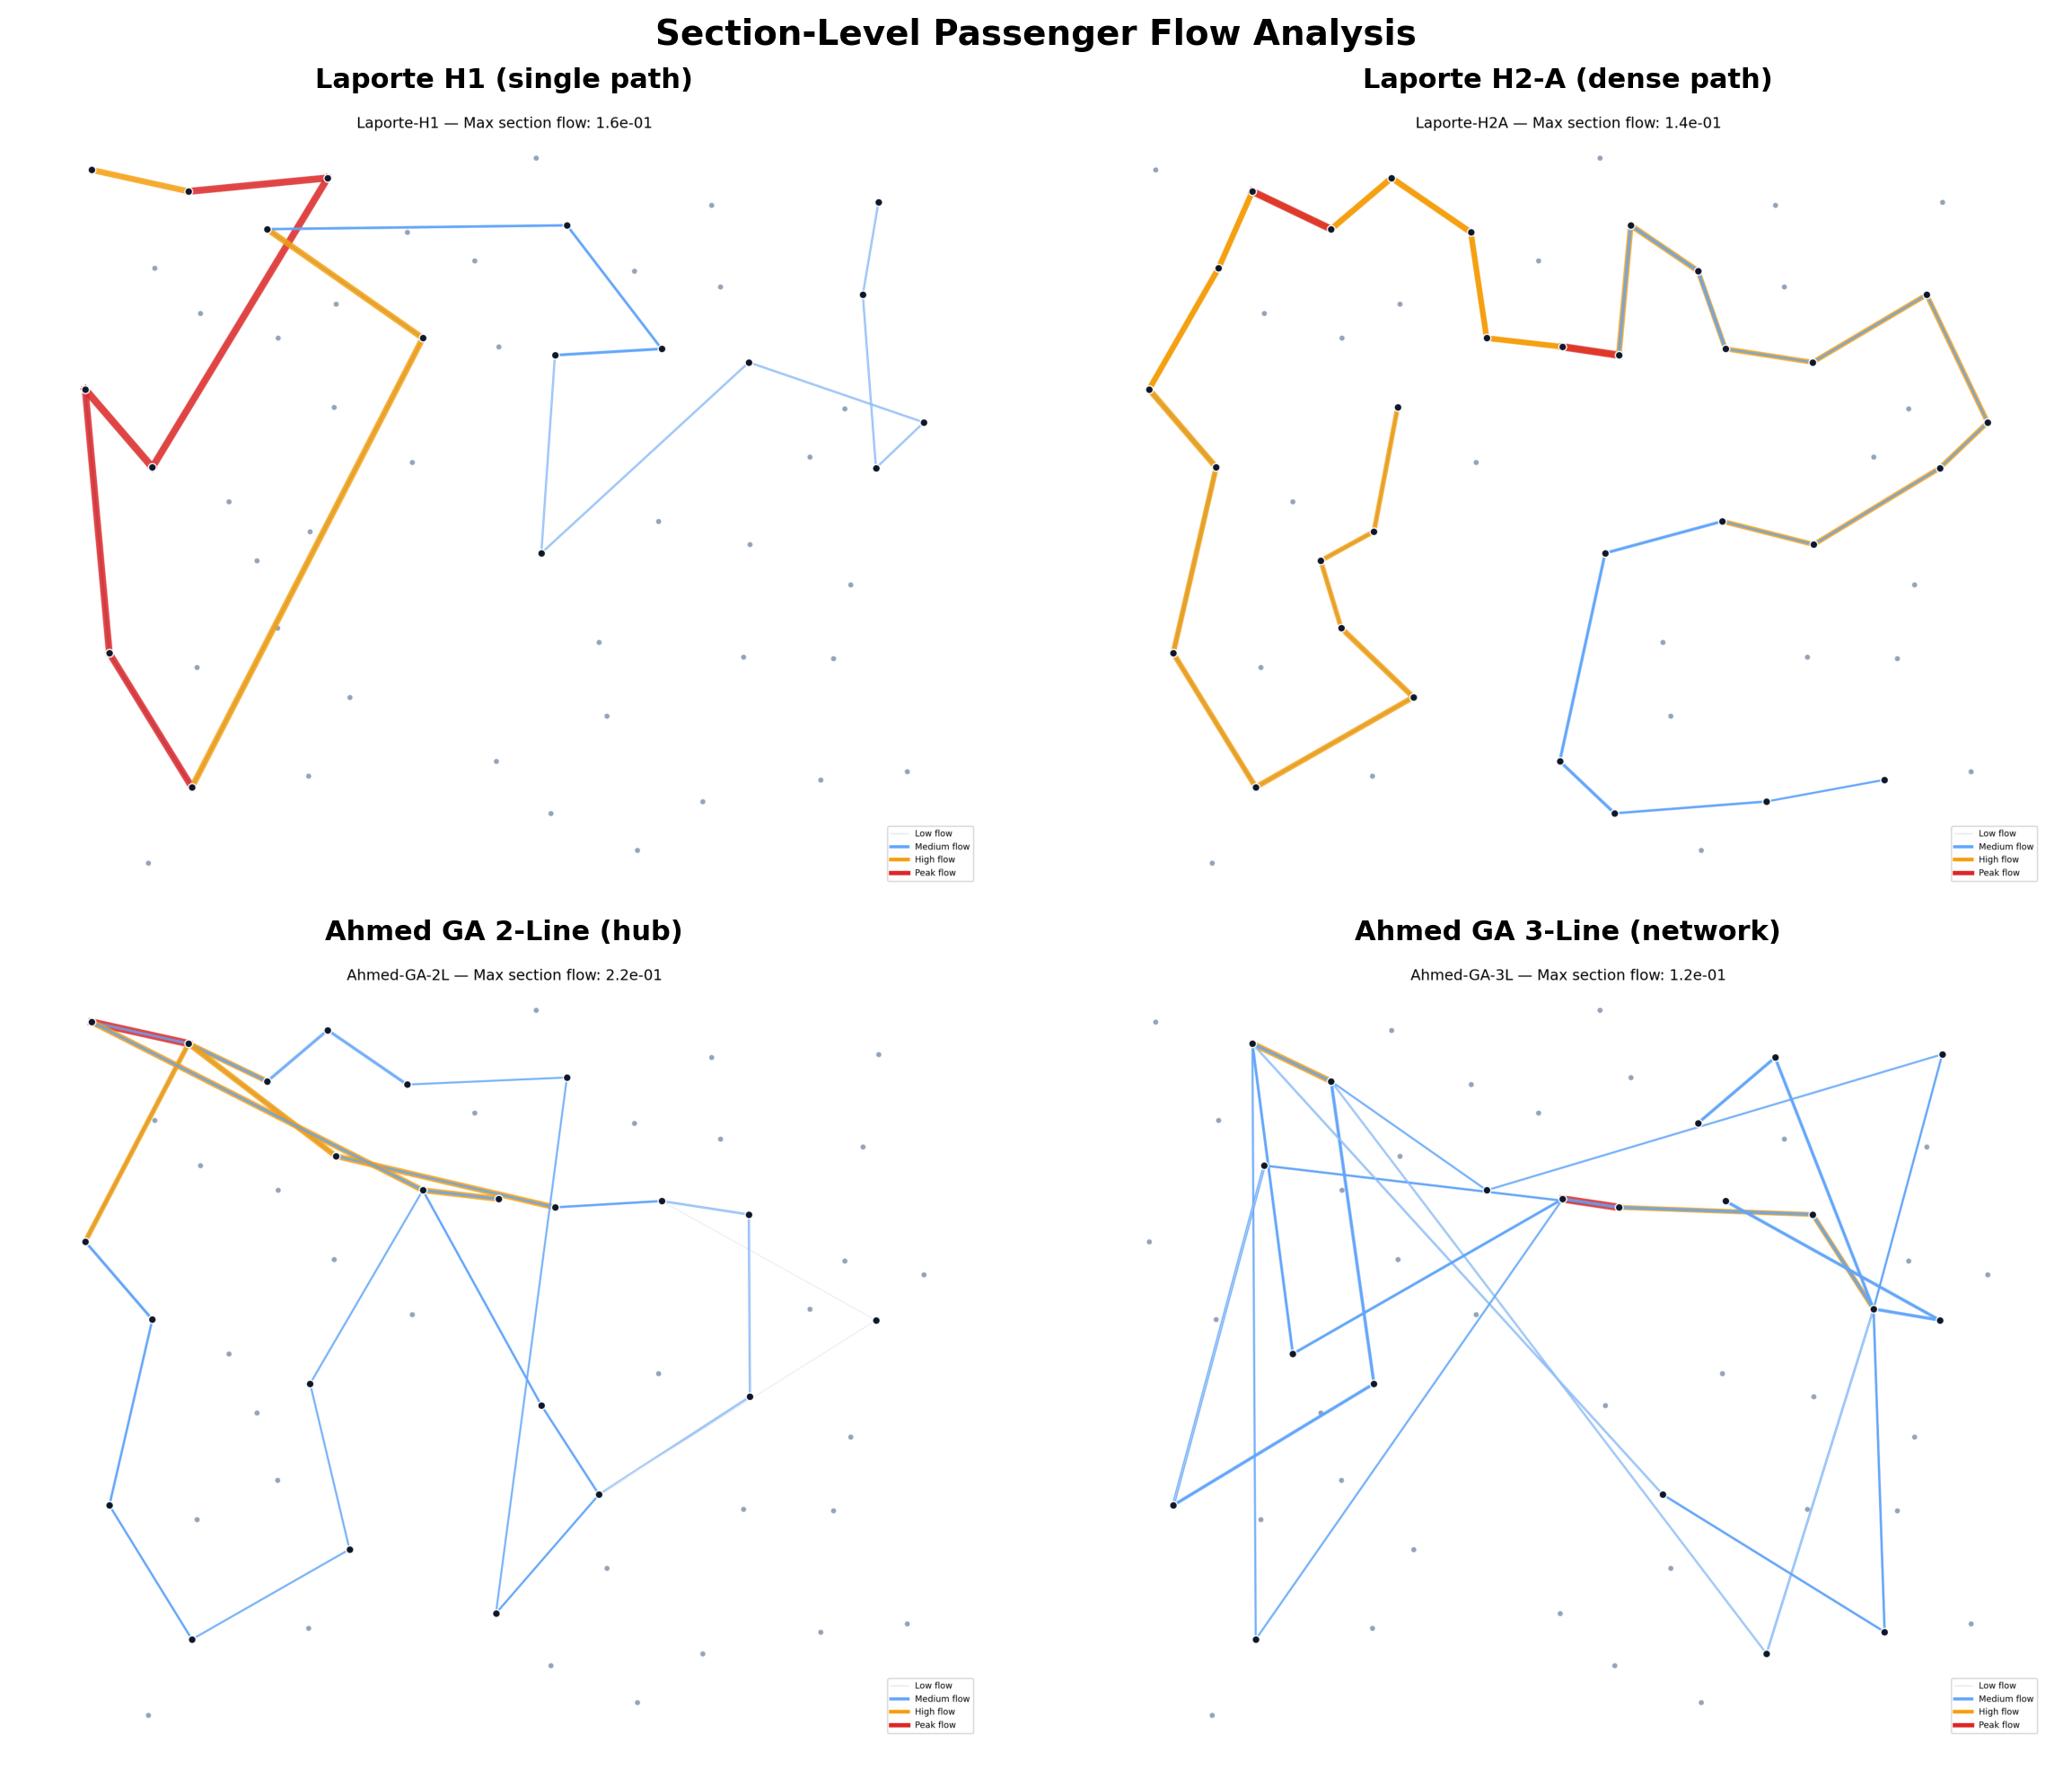
\includegraphics[width=\columnwidth]{figures/flow_comparison.png}
\caption{Passenger flow intensity on four networks (gray=low, blue=medium,
orange=high, red=peak).}
\label{fig:flow_comparison}
\end{figure}

\begin{table}[!htbp]
\centering
\caption{Section-level passenger flow statistics.}
\label{tab:flow}
\scriptsize
\setlength{\tabcolsep}{3pt}
\begin{tabular}{lrrrr}
\toprule
Method & Max Flow & Mean Flow & Top-5 Share & Edges \\
\midrule
Laporte-H1  & 0.16 & 0.033 & 56.9\% & 28/34 \\
Laporte-H2A & 0.14 & 0.045 & 20.3\% & 60/60 \\
Ahmed-GA-2L & 0.22 & 0.027 & 49.9\% & 40/52 \\
Ahmed-GA-3L & 0.12 & 0.016 & 39.4\% & 43/48 \\
\bottomrule
\end{tabular}
\end{table}

\subsection{Sensitivity Analysis}

Spacing sensitivity (500--1,500 m) showed no effect because all corridor
edges exceed 1,000 m---a limitation of our sparse layout. GA convergence
(Fig.~\ref{fig:ahmed_convergence}) stabilizes within 10--15 generations,
confirming the paper's $P_c=0.7$ recommendation.

\begin{figure}[t]
\centering
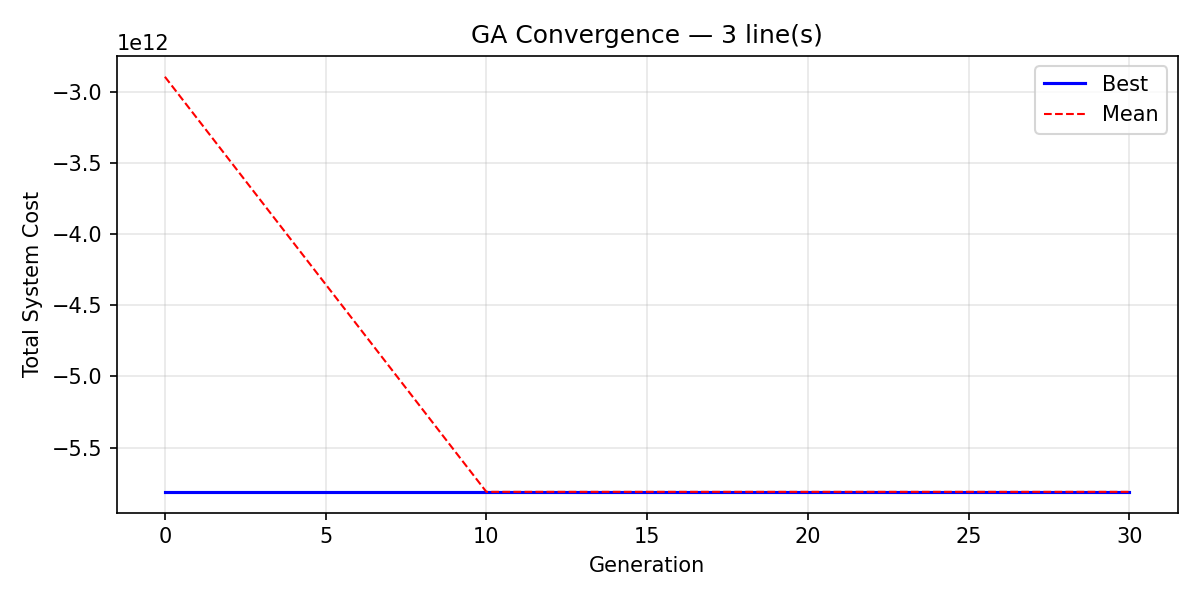
\includegraphics[width=\columnwidth]{figures/ahmed_convergence.png}
\caption{GA convergence for the 3-line scenario.}
\label{fig:ahmed_convergence}
\end{figure}

%--------------------------------------------------------------------------
\section{Conclusion}
%--------------------------------------------------------------------------

This project combines reproduction with a new reduced-search line-planning
framework on a common Shanghai candidate graph. Key findings: (1) the
Laporte reproduction verifies the expected runtime scaling, but our
simplified model (no logit mode choice) reverses the paper's H1-vs-H2
ranking; H2-C achieves the highest OD coverage (56.8\%) by packing more
stations into one alignment. (2) The Ahmed reproduction produces realistic
hub-based multi-line networks; simultaneous optimization outperforms
individual optimization by 18\%. (3) CLPS provides a computationally light
third family of methods: CLPS-Greedy-OD reaches 51.9\% OD coverage in
0.01 s by selecting from a precomputed pool of plausible lines. Together,
the results show that classical constructive heuristics, direct multi-line
GA search, and line-pool selection expose different trade-offs between
coverage, directness, transfers, and runtime. Future work: real OD data,
logit mode choice, and parallel GA evaluation for larger candidate sets.

\bibliographystyle{IEEEtran}
\begin{thebibliography}{99}

\bibitem{laporte2005}
G.~Laporte, J.~A.~Mesa, F.~A.~Ortega, and I.~Sevillano,
``Maximizing trip coverage in the location of a single rapid transit
alignment,'' \emph{Annals of Operations Research}, vol.~136, pp.~299--314,
2005.

\bibitem{ahmed2020}
C.~Ahmed, K.~Nur, and W.~Ochieng,
``GIS and genetic algorithm based integrated optimization for rail transit
system planning,'' \emph{Journal of Rail Transport Planning \& Management},
vol.~16, p.~100222, 2020.

\bibitem{chai2019}
Y.~Chai, Q.~Peng, and J.~Wang,
``Design of urban rail transit network constrained by urban road network,
trips and land-use characteristics,'' \emph{Sustainability}, vol.~11,
no.~21, p.~6128, 2019.

\bibitem{dufourd1996}
H.~Dufourd, M.~Gendreau, and G.~Laporte,
``Locating a transit line using Tabu search,'' \emph{Location Science},
vol.~4, no.~1, pp.~1--19, 1996.

\bibitem{bruno2002}
G.~Bruno, M.~Gendreau, and G.~Laporte,
``A heuristic for the location of a rapid transit line,''
\emph{Computers \& Operations Research}, vol.~29, no.~1, pp.~1--12, 2002.

\bibitem{schoebel2005}
A.~Sch\"{o}bel and S.~Scholl,
``Line planning with minimal traveling time,''
in \emph{ATMOS 2005}, 2005.

\bibitem{vuchic1968}
V.~R.~Vuchic and G.~F.~Newell,
``Rapid transit interstation spacings for minimum travel time,''
\emph{Transportation Science}, vol.~2, no.~4, pp.~303--339, 1968.

\bibitem{gutierrez2013}
G.~Guti\'{e}rrez-Jarpa, C.~Obreque, G.~Laporte, and V.~Marianov,
``Rapid transit network design for optimal cost and origin-destination
demand capture,'' \emph{Computers \& Operations Research}, vol.~40,
no.~12, pp.~3000--3009, 2013.

\end{thebibliography}

\end{document}
